\section{Implementation}
\label{sec:implementation}

\subsection{Client and Server Communication}
Our client is written in JavaScript and uses SoundManager, a
JavaScript audio player API. In contrast, our server code is
written in Python 2.7. Both use the Google App Engine API. 

When the client wants to contact the server, it issues an HTTP
request, which is handled by the appropriate Python script handler.
Handlers in Google App Engine can only serve requests within a
time limit, which is why we chose to store session data within
the Datastore.

In contrast, when the server wants to contact a client, is uses 
the Channel service. Channels are persistent connections that 
allow updates to propagate to clients without the use of polling.
This is the mechanism with which we send updates to participants
of a session. A channel is created as follows: 
\begin{enumerate}
  \item The client contacts the server
  \item The server generates a channel ID and sends back a token
  \item The client connects to the channel using the token
\end{enumerate}
The client receives updates by listening on the channel by opening
a socket and does appropriate actions based on the message received.
Updates to the channel are made via HTTP requests from clients. When
a client disconnects from the channel, a message containing the 
corresponding channel ID is sent to the server, and appropriate
cleanup is performed.	

\subsection{Session Synchronization}
\label{sec:sync}

\begin{figure}[b!]
	\centering
	\begin{subfigure}[b]{0.5\textwidth}
		\centering
		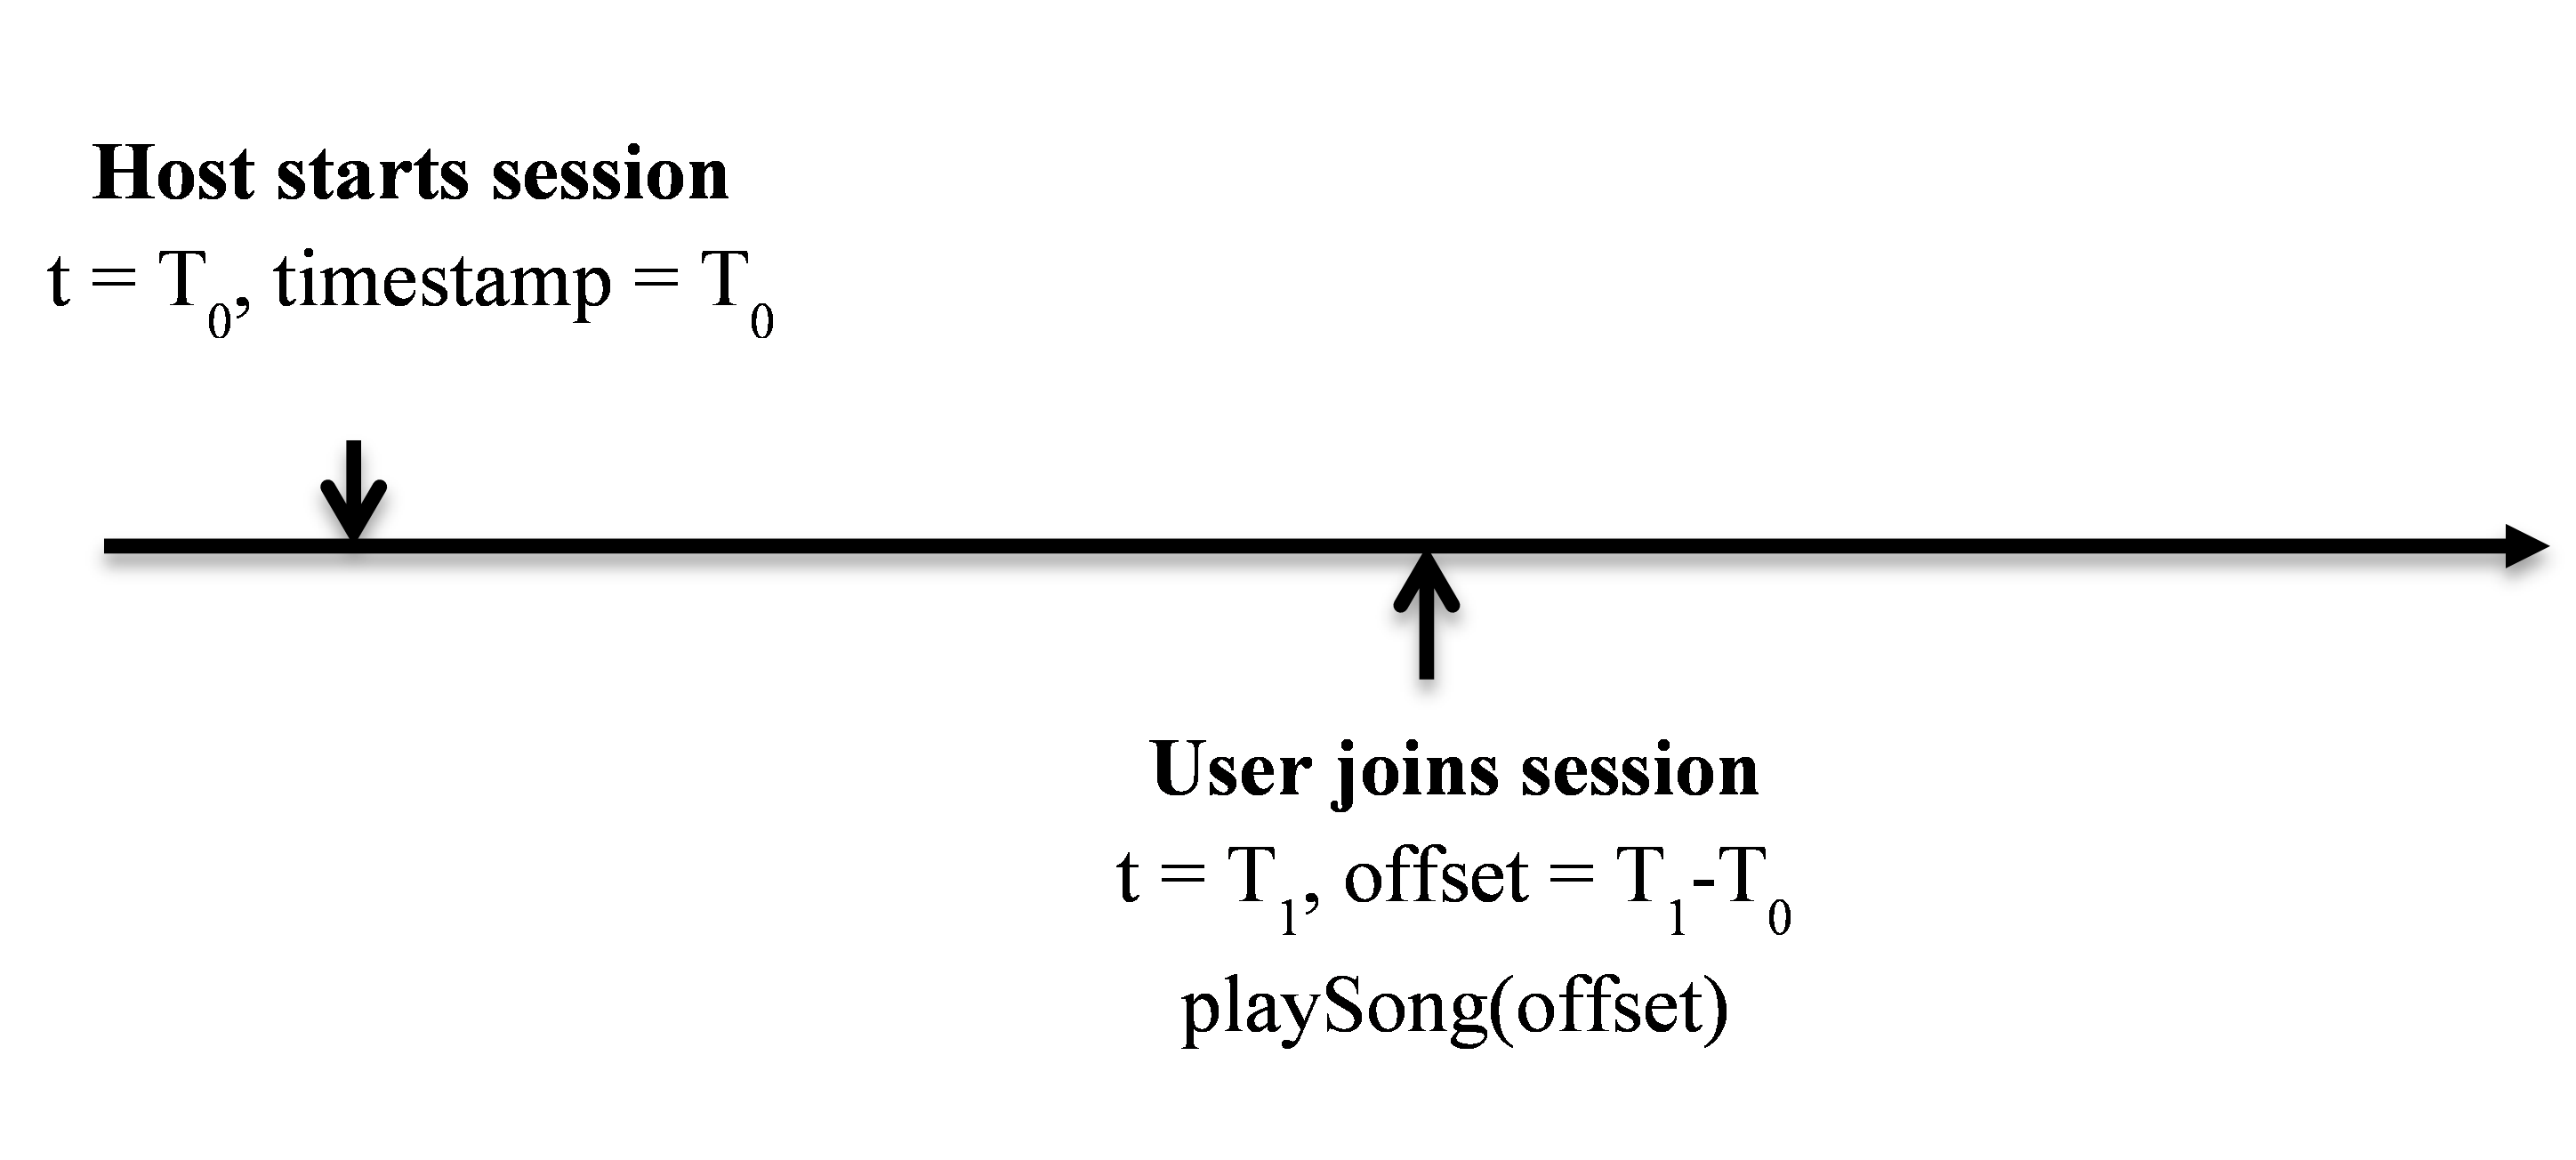
\includegraphics[width=85mm]{joinSessionPlay.png}
		\caption{Joining a session while a song is playing}
		\label{fig:syncJoinPlay}
	\end{subfigure}
	
	\begin{subfigure}[b]{0.5\textwidth}
		\centering
		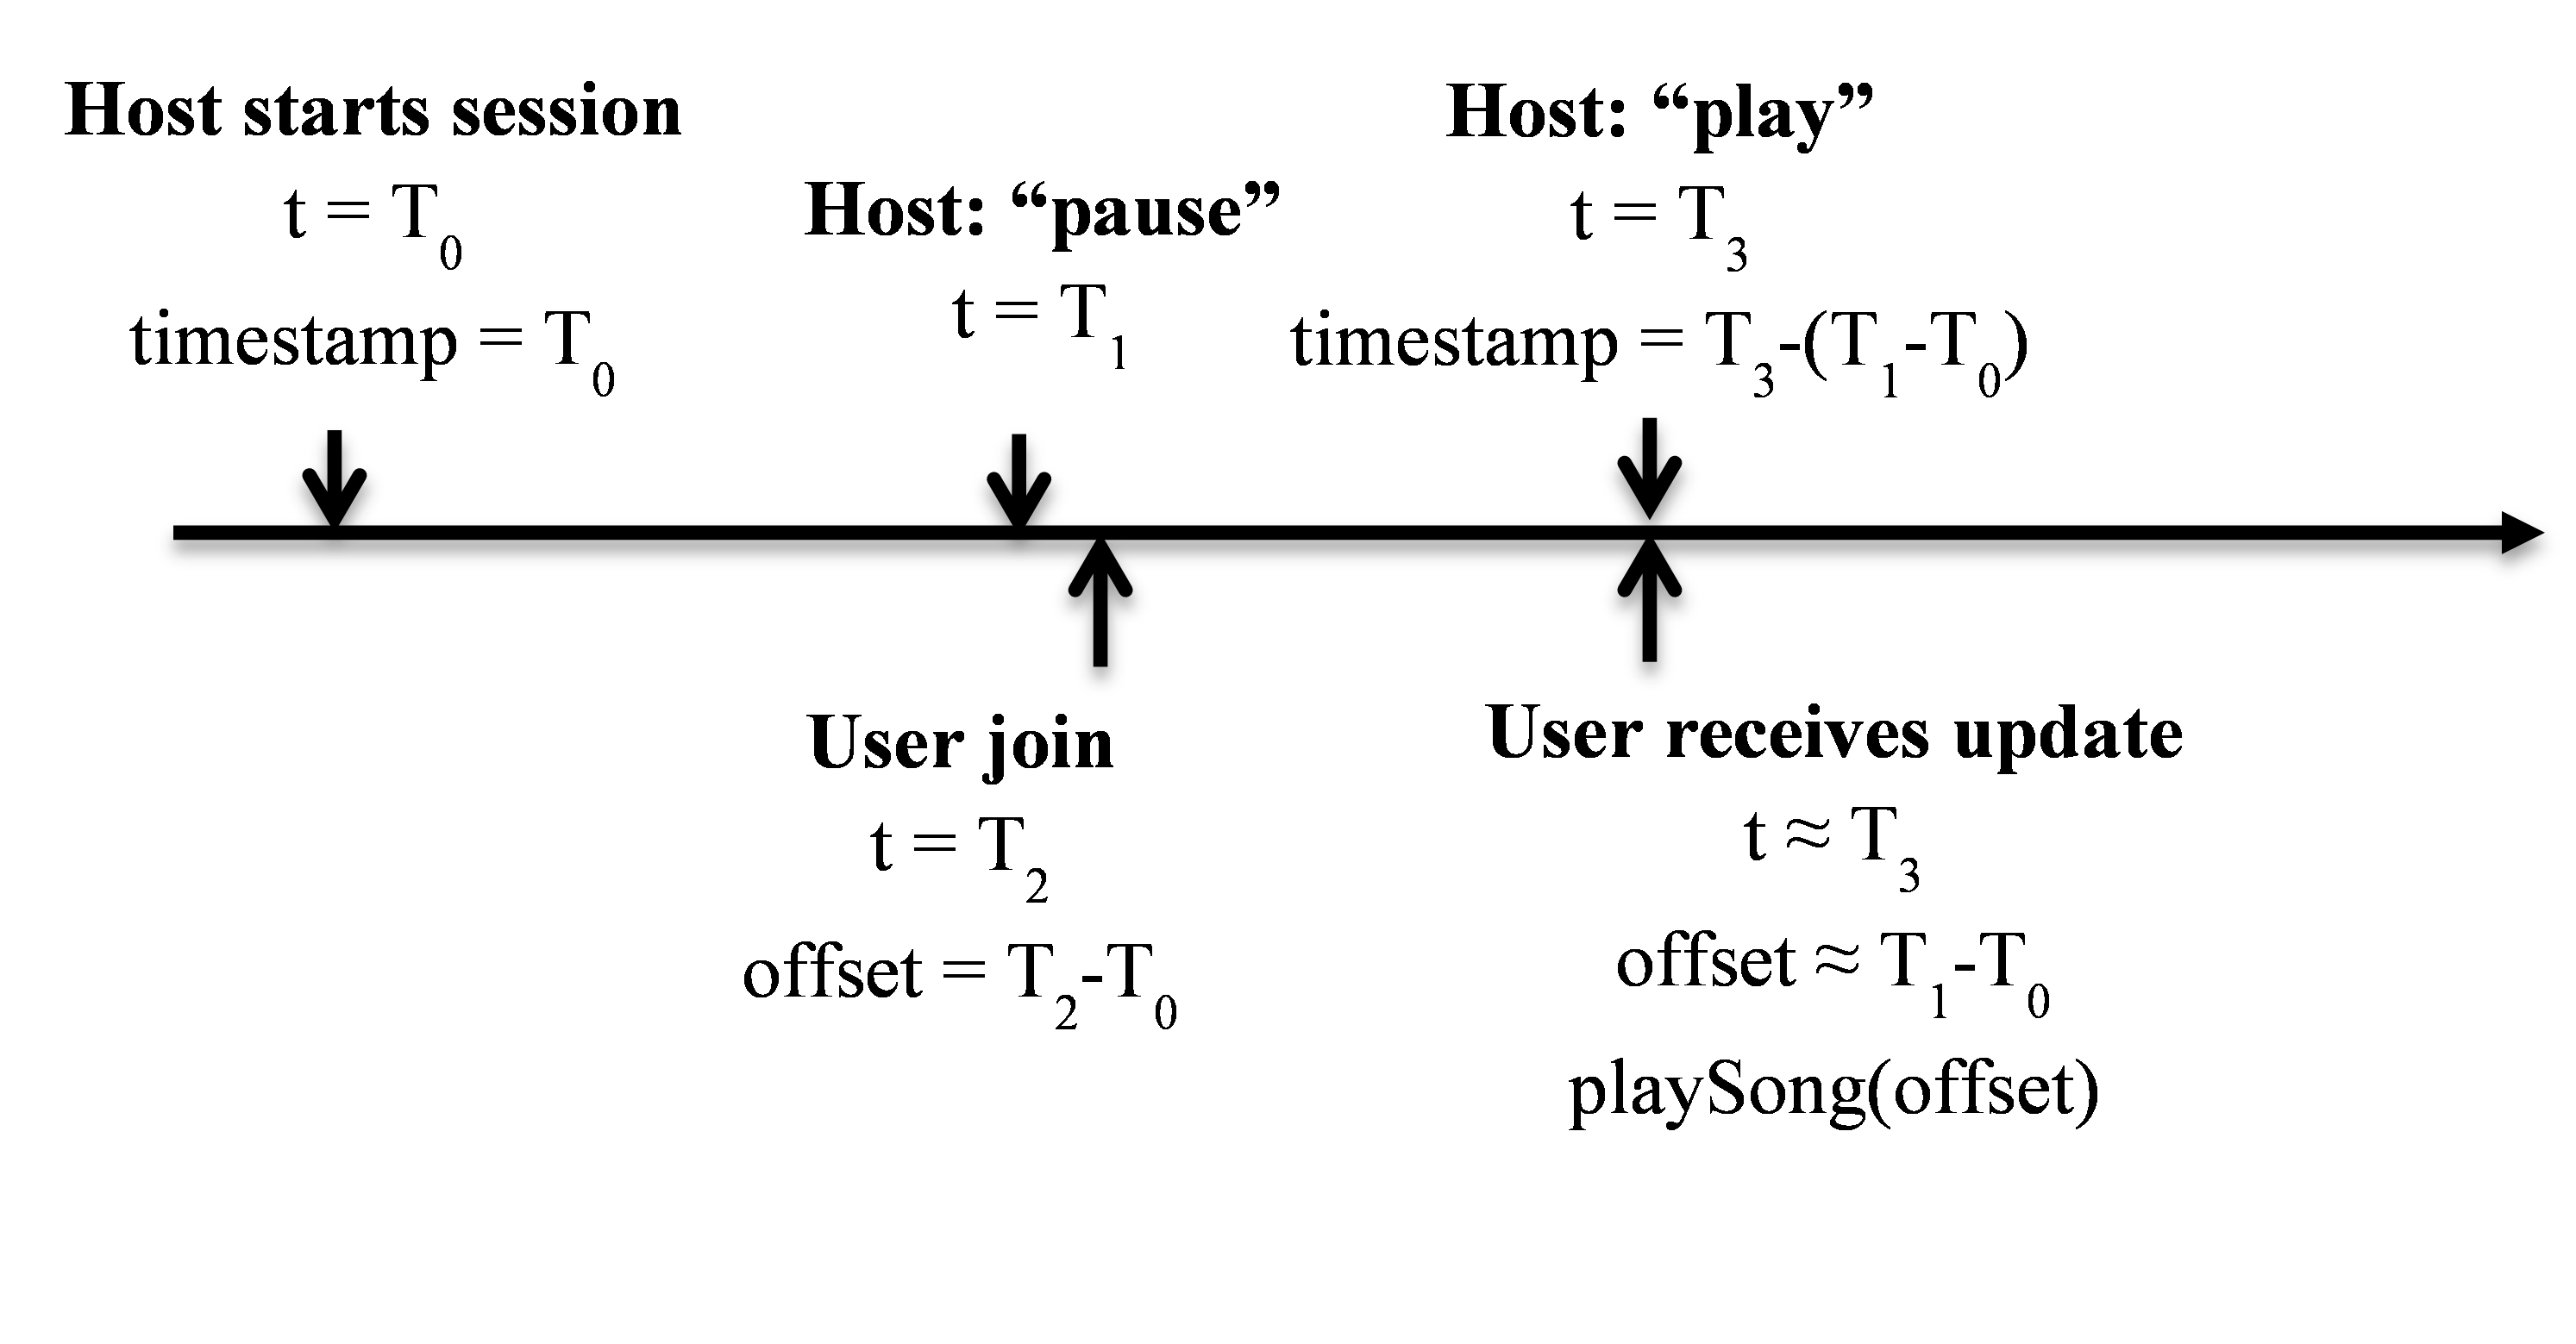
\includegraphics[width=85mm]{joinSessionPause.png}
		\caption{Joining a session while a song is paused}
		\label{fig:syncJoinPause}
	\end{subfigure}
	\caption{Synchronization messages when a user joins a session}
	\label{fig:syncJoin}
\end{figure}

In order to synchronize playback among different clients, we use 
control messages, which are propagated via channels as described
above. Only hosts may issue commands such as play, pause, and 
next for the session. The ``play'' and ``pause'' commands are sent
only when the host clicks on the pause and play buttons, and the 
``next'' command is sent when the host switches songs or if the
host clicks on the ``next'' button. We separate the problem of synchronization 
into two parts: joining an existing session and updating the
current session. In both cases we utilize a timestamp, which is 
updated each time a play or next command is sent by the host client
and is sent with the control message. 

As seen in Figure~\ref{fig:syncJoin} when a user joins a session, 
the server sends the user the elapsed time since the last stored timestamp. 
The user then starts the song with the value returned by the server as 
the offset. If the song is playing when the user joins the session, 
it will start playing at the specified offset. If the song is paused when 
the user joins the session, the retrieved offset will not be the correct 
elapsed time; however, this is corrected when the host sends a ``play'' 
message to the server, which stores another timestamp and propagates
the correct offset to all session listeners.

This timestamping synchronization is used mainly when a user joins a session.
In the other case where participants update their current session upon 
recieving a control message, the offset can usually be inferred based on the local state. 
For instance, if the user receives a ``next'' message, then they
start the next song with an offset of 0. If a user receives a ``pause" 
message, they stop the current song and keep the elapsed time as the offset.
If the user receives a ``play'' message they start the current song at the 
local offset, which was set when the ``pause'' message was received. The exception to this 
is if the current paused song is at the beginning, indicating
that this user has joined the session while the song was paused or that this user is
ahead of the host and is waiting for a control message from the host. 
In this case the user adjusts the current song offset with what 
they recieve from the server. Conversely, if the listener lags behind the host, then they will
receive a ``next'' message before the end of the song and start the next song. Figure~\ref{fig:syncUsers}
illustrates the timeline in the cases where a listener is behind the host and where a listener
is ahead of the host.

\begin{figure}[t!]
	\centering
	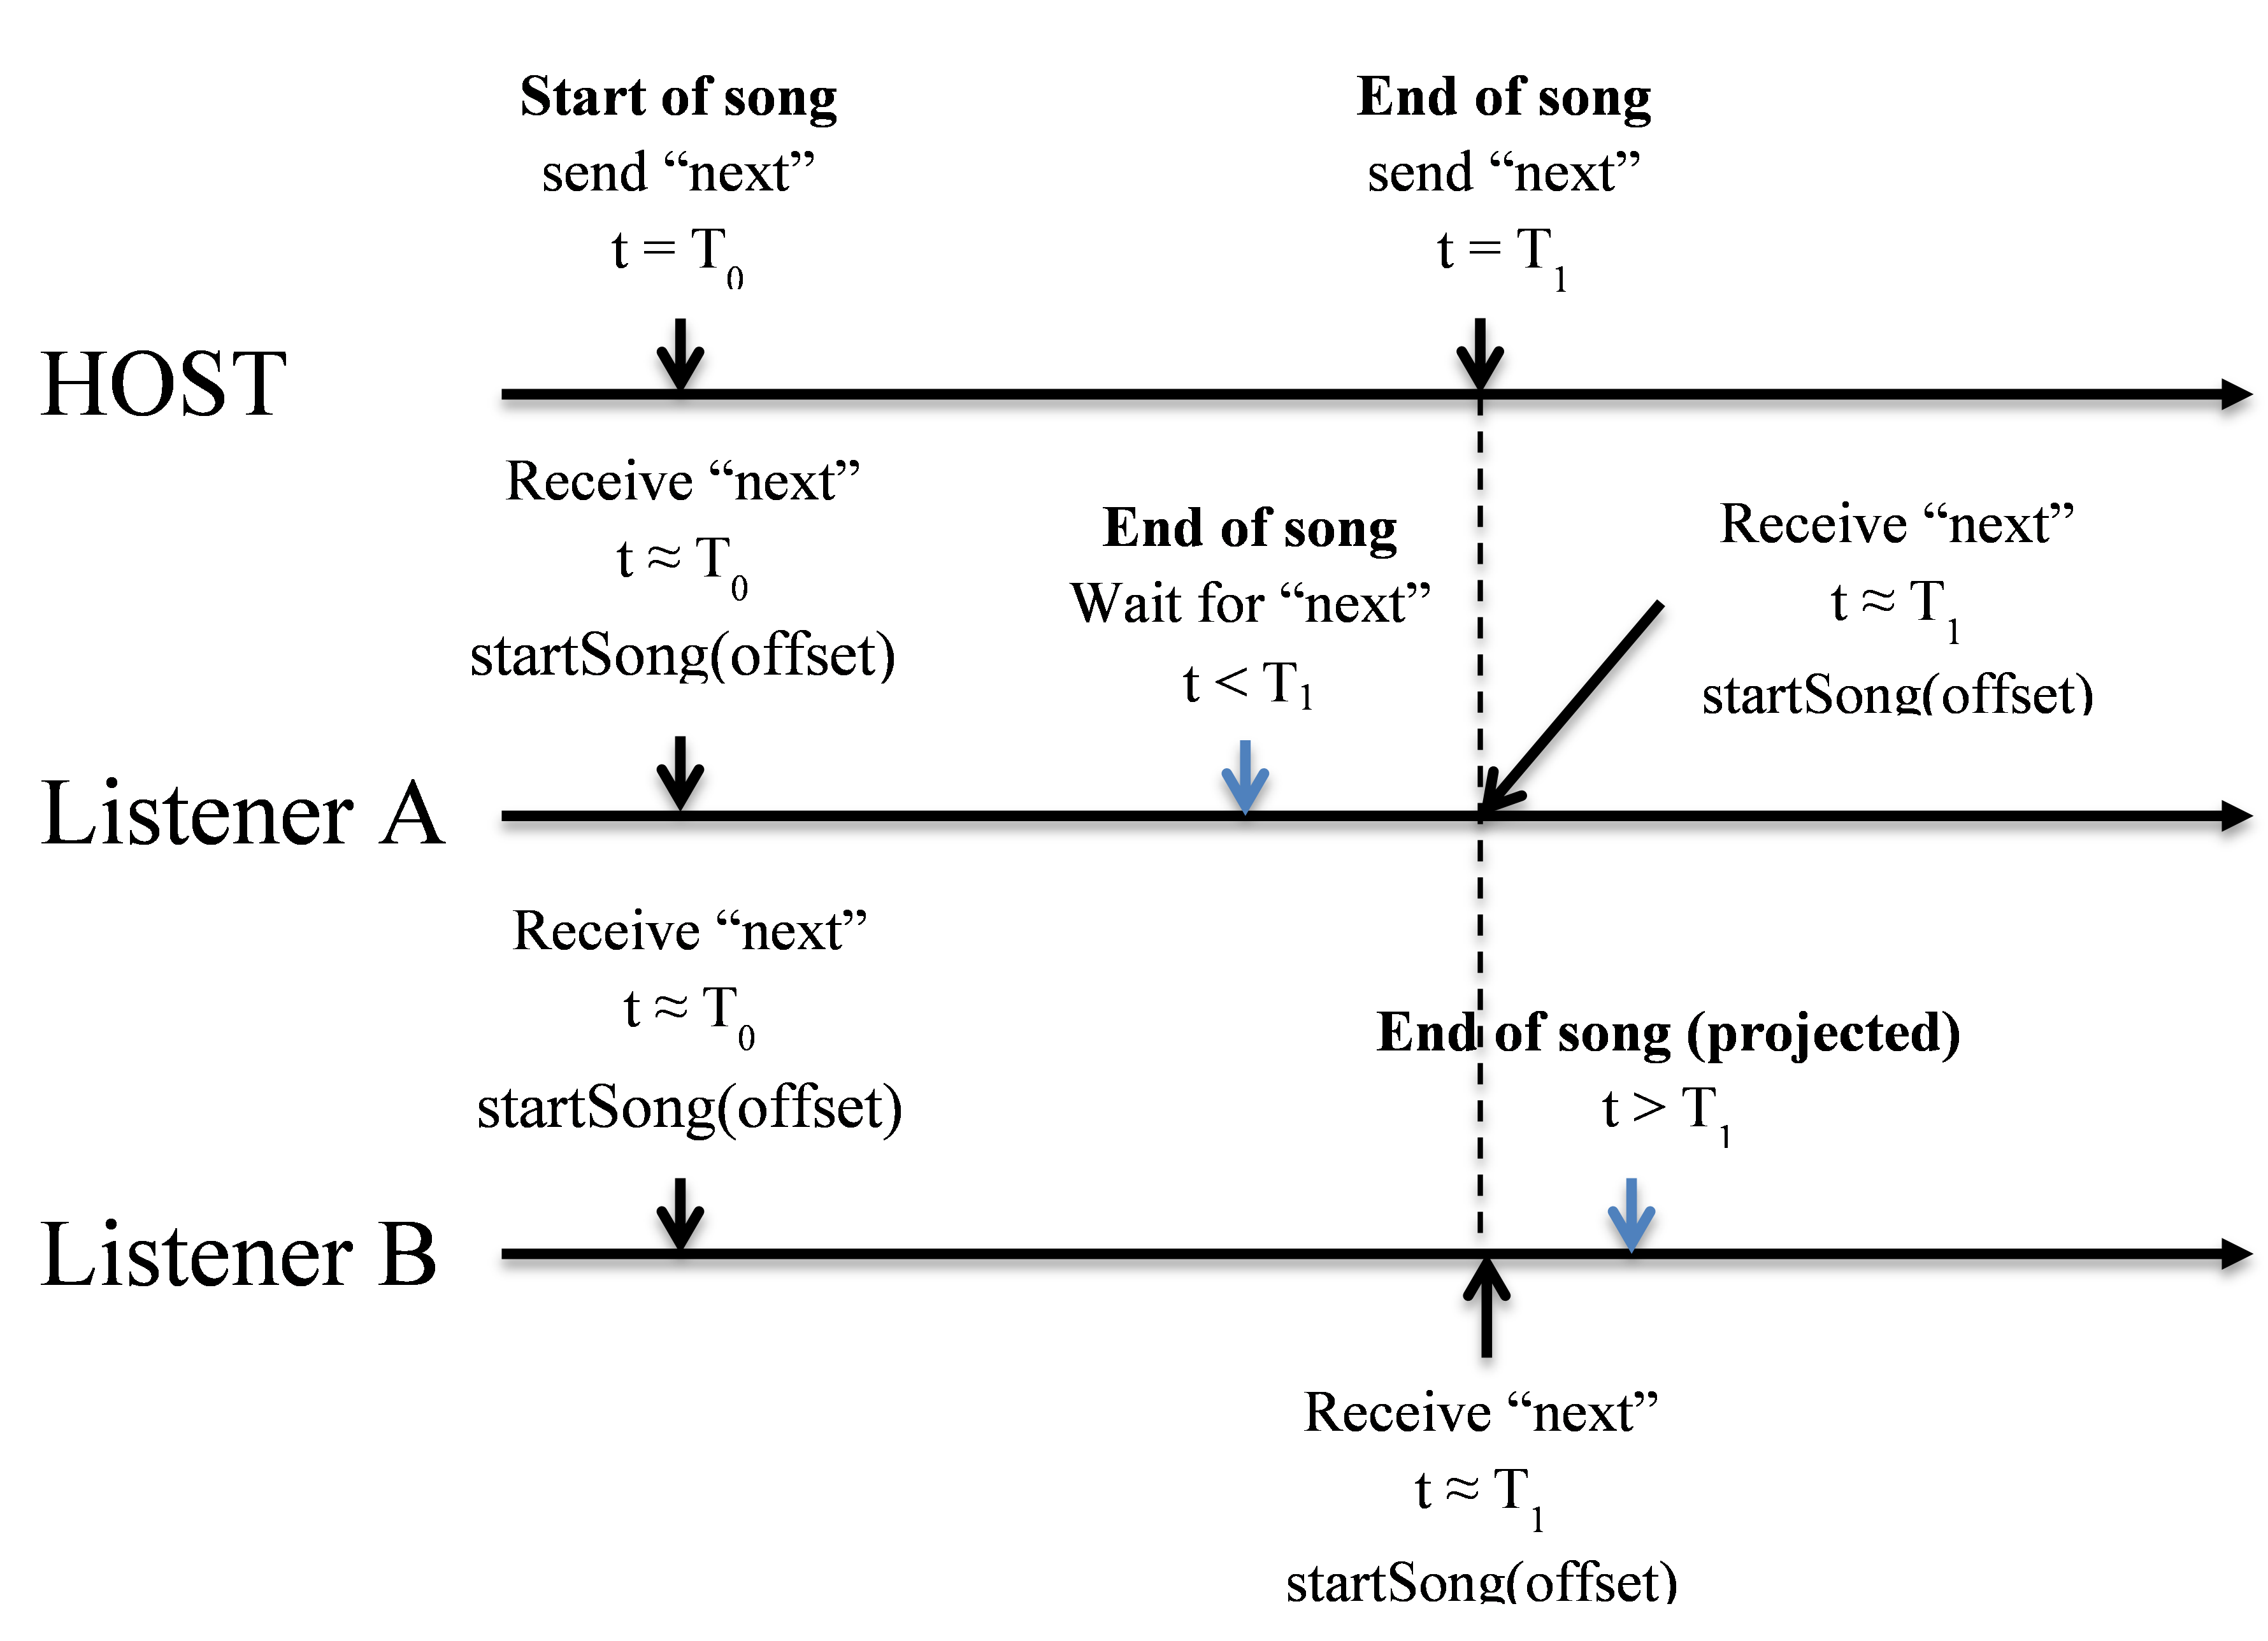
\includegraphics[width=85mm]{syncSessionUsers.png}
	\caption{The synchronization timeline for a listener that's ahead of or behind the host}
	\label{fig:syncUsers}
\end{figure}


\section{Design Considerations}
\label{sec:considerations}
We made certain design decisions in order to achieve the goals discussed
in Section~\ref{sec:intro}. In this section we summarize and discuss these choices.
\begin{enumerate}
  \item \textbf{Performance}: Songs are prefetched by the client for seemless transitions. 
  		We also perform synchronization, as discussed in Section~\ref{sec:sync}.
  \item \textbf{Availability}: We rely on Google services such as 
  		Datastore and Blobstore, which are highly replicated and reliable. Requests are
  		also served as long as Google App Engine is available. We discuss how our system
		behaves with various failure modes in Section~\ref{sec:faultTolerance}.
  \item \textbf{Scalability}: For scalability purposes, we allow concurrent requests.
  		To minimize the number and size of messages, we allow incremental
  		updates. We do not send all session data on an update
\end{enumerate}

\subsection{Fault Tolerance}
\label{sec:faultTolerance}
There are several components of our system that could fail. The host or listener
of a session could lose connection to the server or the master/session server
could go down. We discuss each type of
failure below with respect to the impact on other users of the system.

When the host of a session goes down, the system mainly continues
to operate as normal. Any listeners in the session of the down host
will continue playing the current song until completion. At that
time, they will wait until the host reconnects and updates the
session server with new information. Other clients will still be
able to join the session, but will have to wait like the current
listeners. Once the host reconnects, it rejoins its hosted session
and continues playback as if it just joined the session.

A listener losing connection has very little impact on the system. The session
server will detect the channel failure and cleanup necessary state
associated with the listener. Other listeners as well as the host
of the session will not be impacted by the disconnected listener.

When the master server fails, active sessions continue to
operate as before. Hosts and listeners can continue to listen
together to existing and newly added songs. However, new clients
attempting to connect to the system will have their requests time
out because the master server handles all initial client connections.

If the session server fails, all session updates will fail.
Clients will finish the current song of their session and then
will have to wait for the session server to come back up. New clients
first connecting to the system will be able to login, but will not
be able to join a session. They will also be unable to start a session until
the session server comes back up.